\chapter{Relationships}\label{relationships}

This chapter explores relationships between variables.

\begin{itemize}
\item
  We will visualize relationships using scatter plots, box plots, and
  violin plots,
\item
  And we will quantify relationships using correlation and simple
  regression.
\end{itemize}

The most important lesson in this chapter is that you should always
visualize the relationship between variables before you try to quantify
it -- otherwise, you are likely to be misled.

\section{Exploring relationships}\label{exploring-relationships}

So far we have mostly considered one variable at a time. Now it's time
to explore relationships between variables. As a first example, we'll
look at the relationship between height and weight. We'll use data from
the Behavioral Risk Factor Surveillance System (BRFSS), which is run by
the Centers for Disease Control. Based on the BRFSS data from 2021, I
have created an extract with one row for each survey respondent and one
column for each of the variables I selected.

\begin{lstlisting}[language=Python,style=source]
import pandas as pd

brfss = pd.read_hdf('brfss_2021.hdf', 'brfss')
brfss.shape
\end{lstlisting}

\begin{lstlisting}[style=output]
(438693, 10)
\end{lstlisting}

Here are the first few rows.

\begin{lstlisting}[language=Python,style=source]
brfss.drop(columns='SEQNO').head()
\end{lstlisting}

\begin{tabular}{lrrrrrrrrr}
\midrule
 & HTM4 & WTKG3 & \_SEX & \_AGEG5YR & \_VEGESU1 & \_INCOMG1 & \_LLCPWT & \_HTM4G10 & AGE \\
\midrule
0 & 150.000000 & 32.660000 & 2 & 11.000000 & 2.140000 & 3.000000 & 744.745531 & 140.000000 & 72.000000 \\
1 & 168.000000 & NaN & 2 & 10.000000 & 1.280000 & NaN & 299.137394 & 160.000000 & 67.000000 \\
2 & 165.000000 & 77.110000 & 2 & 11.000000 & 0.710000 & 2.000000 & 587.862986 & 160.000000 & 72.000000 \\
3 & 163.000000 & 88.450000 & 2 & 9.000000 & 1.650000 & 5.000000 & 1099.621570 & 160.000000 & 62.000000 \\
4 & 180.000000 & 93.440000 & 1 & 12.000000 & 2.580000 & 2.000000 & 1711.825870 & 170.000000 & 77.000000 \\
\midrule
\end{tabular}

The BRFSS includes hundreds of variables. For the examples in this
chapter, we'll work with just these nine. The ones we'll start with are
\passthrough{\lstinline!HTM4!}, which records each respondent's height
in centimeters, and \passthrough{\lstinline!WTKG3!}, which records
weight in kilograms.

\begin{lstlisting}[language=Python,style=source]
height = brfss['HTM4']
weight = brfss['WTKG3']
\end{lstlisting}

To visualize the relationship between these variables, we'll make a
\textbf{scatter plot}, which shows one marker for each pair of values.
Scatter plots are common and readily understood, but they are
surprisingly hard to get right. As a first attempt, we'll use
\passthrough{\lstinline!plot!} with the style string
\passthrough{\lstinline!o!}, which plots a circle for each data point.

\begin{lstlisting}[language=Python,style=source]
import matplotlib.pyplot as plt

plt.plot(height, weight, 'o')

plt.xlabel('Height in cm')
plt.ylabel('Weight in kg')
plt.title('Scatter plot of weight versus height');
\end{lstlisting}

\begin{center}
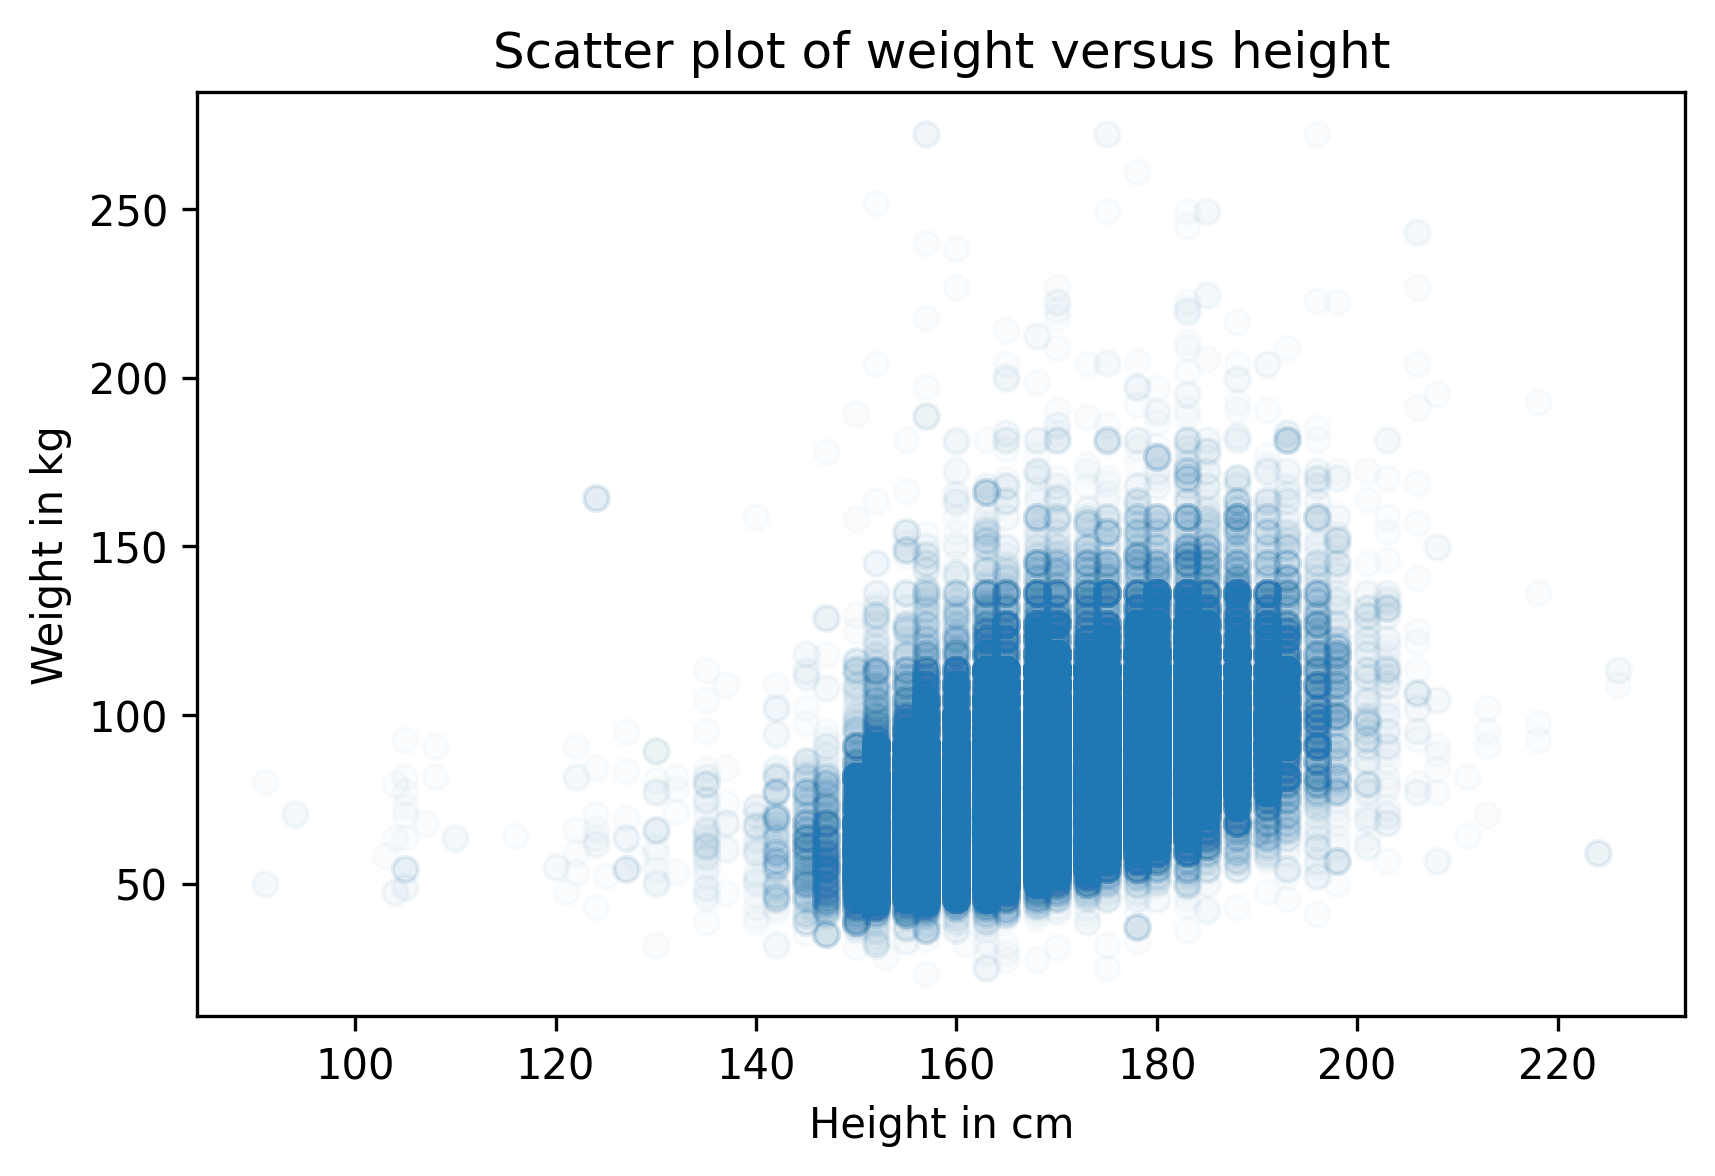
\includegraphics[width=4in]{chapters/09_relationships_files/09_relationships_14_0.png}
\end{center}

Each marker represents the height and weight of one person. Based on the
shape of the result, it looks like taller people are heavier, but there
are a few things about this plot that make it hard to interpret. Most
importantly, it is \textbf{overplotted}, which means that there are
markers piled on top of each other so you can't tell where there are a
lot of data points and where there is just one. When that happens, the
picture can be misleading.

One way to improve the plot is to use transparency, which we can do with
the keyword argument \passthrough{\lstinline!alpha!}. The lower the
value of alpha, the more transparent each data point is.\\
Here's what it looks like with \passthrough{\lstinline!alpha=0.01!}.

\begin{lstlisting}[language=Python,style=source]
plt.plot(height, weight, 'o', alpha=0.01)

plt.xlabel('Height in cm')
plt.ylabel('Weight in kg')
plt.title('Scatter plot of weight versus height');
\end{lstlisting}

\begin{center}
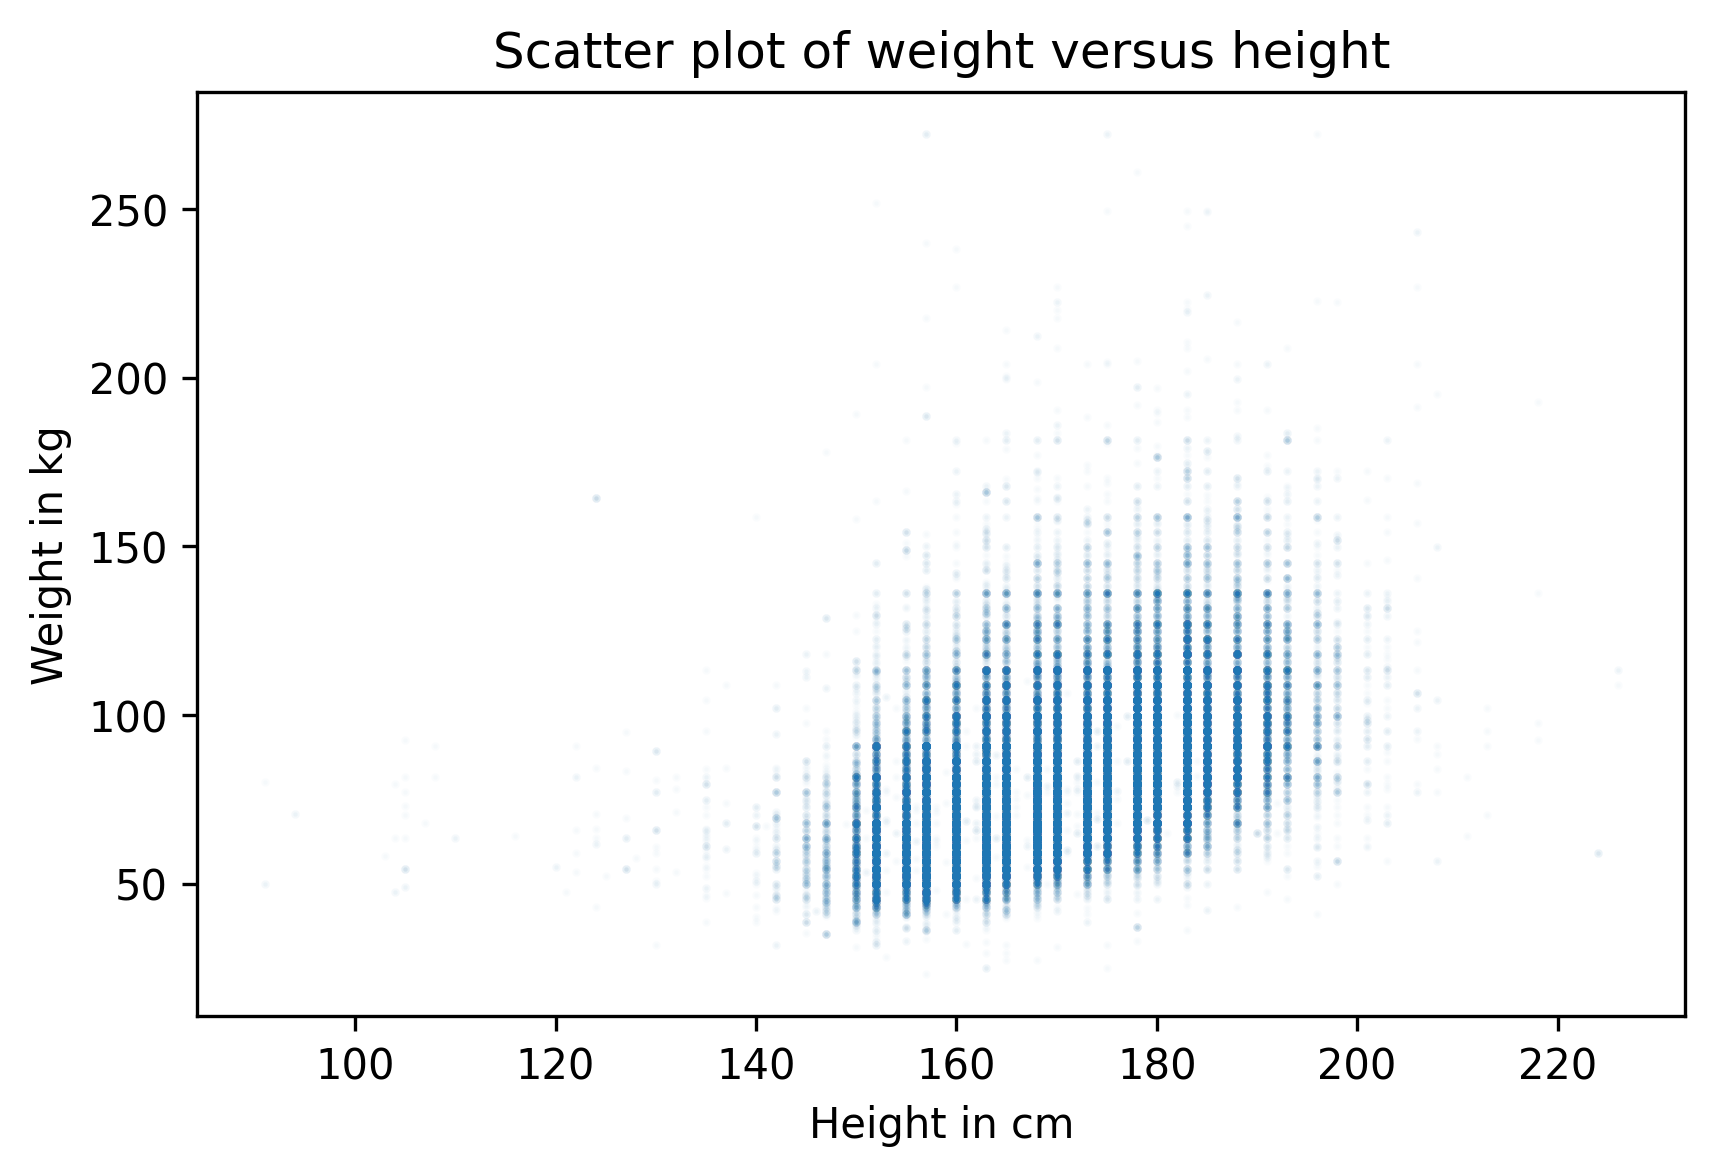
\includegraphics[width=4in]{chapters/09_relationships_files/09_relationships_16_0.png}
\end{center}

This is better, but there are so many data points, the scatter plot is
still overplotted. The next step is to make the markers smaller. With
\passthrough{\lstinline!markersize=0.5!} and a low value of alpha, the
scatter plot is less saturated. Here's what it looks like.

\begin{lstlisting}[language=Python,style=source]
plt.plot(height, weight, 'o', alpha=0.01, markersize=0.5)

plt.xlabel('Height in cm')
plt.ylabel('Weight in kg')
plt.title('Scatter plot of weight versus height');
\end{lstlisting}

\begin{center}
\includegraphics[width=4in]{chapters/09_relationships_files/09_relationships_18_0.png}
\end{center}

Again, this is better, but now we can see that the points fall in
discrete columns. That's because most heights were reported in inches
and converted to centimeters. We can break up the columns by adding
random noise to the values, which is called \textbf{jittering}. We'll
can use NumPy to generate noise from a normal distribution with mean 0
and standard deviation 2.

\begin{lstlisting}[language=Python,style=source]
import numpy as np

noise = np.random.normal(0, 2, size=len(brfss))
height_jitter = height + noise
\end{lstlisting}

Here's what the plot looks like with jittered heights.

\begin{lstlisting}[language=Python,style=source]
plt.plot(height_jitter, weight, 'o', alpha=0.01, markersize=0.5)

plt.xlabel('Height in cm')
plt.ylabel('Weight in kg')
plt.title('Scatter plot of weight versus height');
\end{lstlisting}

\begin{center}
\includegraphics[width=4in]{chapters/09_relationships_files/09_relationships_22_0.png}
\end{center}

The columns are gone, but now we can see that there are rows where
people rounded off their weight. We can fix that by jittering weight,
too.

\begin{lstlisting}[language=Python,style=source]
noise = np.random.normal(0, 2, size=len(brfss))
weight_jitter = weight + noise
\end{lstlisting}

Here's what it looks like.

\begin{lstlisting}[language=Python,style=source]
plt.plot(height_jitter, weight_jitter, 'o', 
         alpha=0.01, markersize=0.5)

plt.xlabel('Height in cm')
plt.ylabel('Weight in kg')
plt.title('Scatter plot of weight versus height');
\end{lstlisting}

\begin{center}
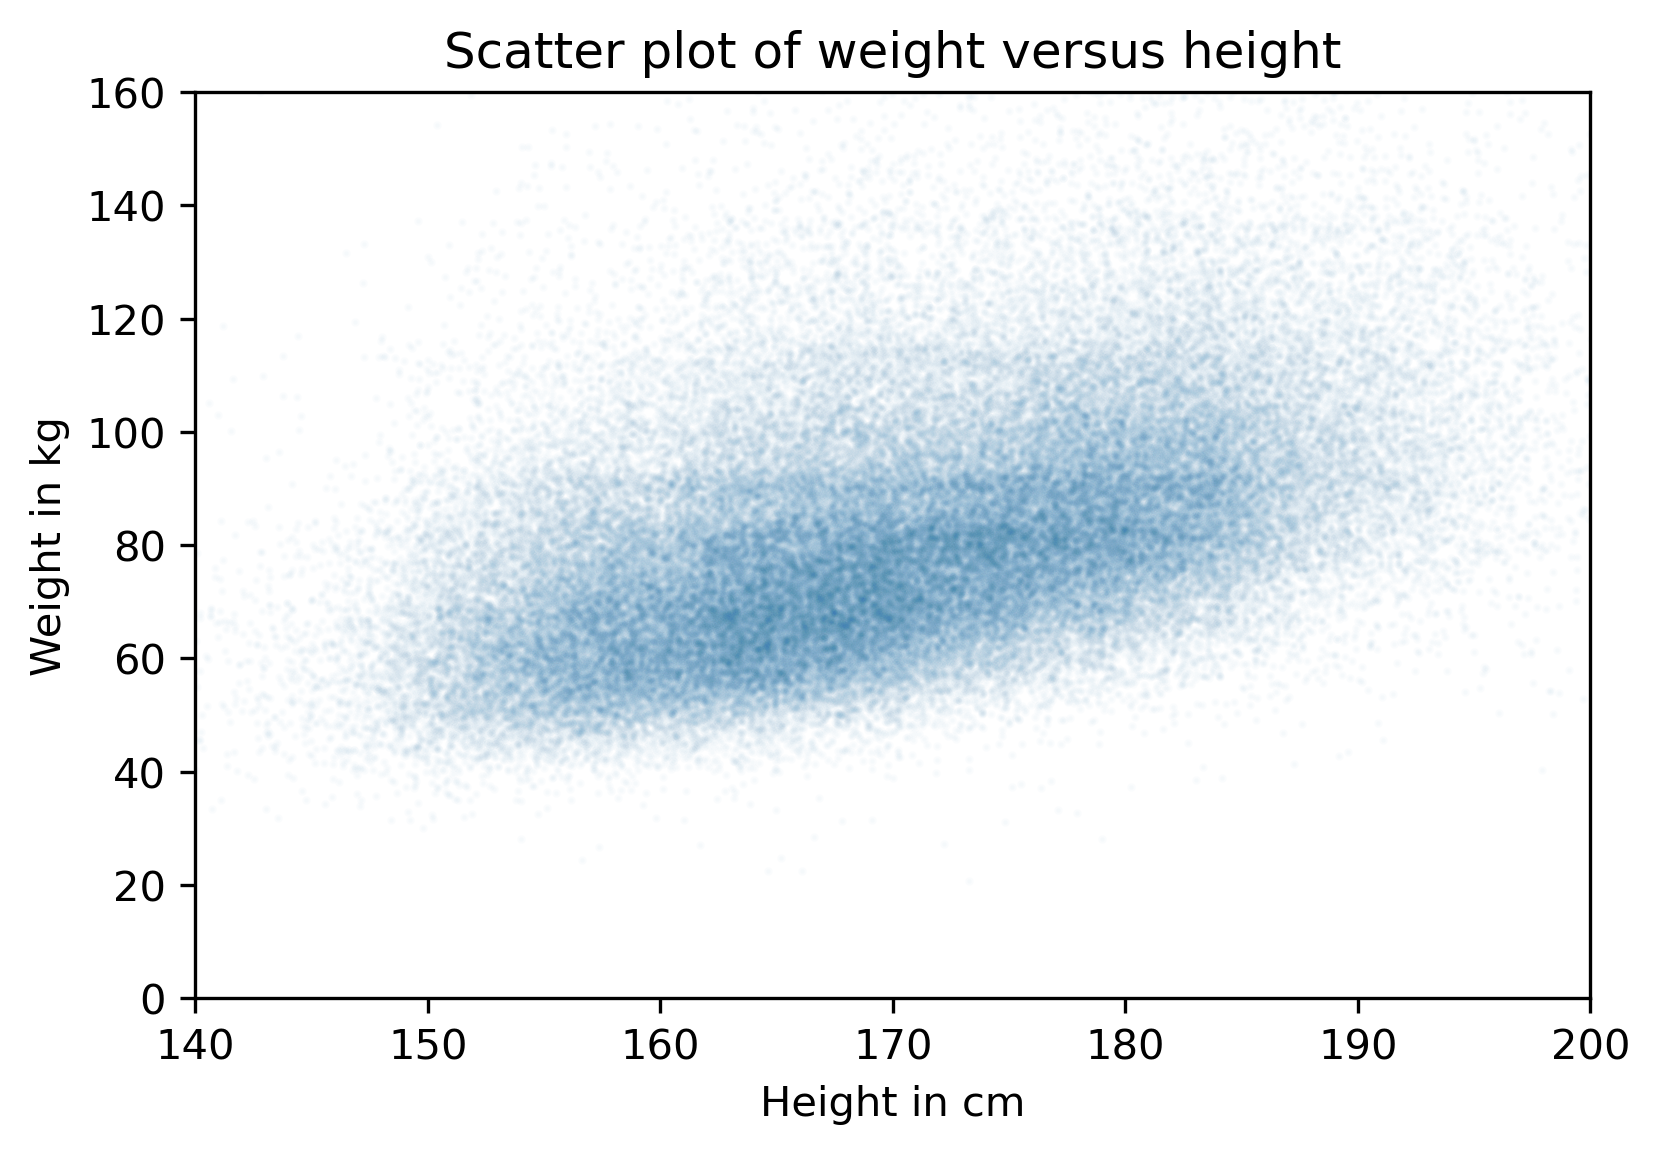
\includegraphics[width=4in]{chapters/09_relationships_files/09_relationships_26_0.png}
\end{center}

Finally, let's zoom in on the area where most of the data points are.
The functions \passthrough{\lstinline!xlim!} and
\passthrough{\lstinline!ylim!} set the lower and upper limits of the
x-axis and y-axis; in this case, we plot heights from 140 to 200
centimeters and weights up to 160 kilograms. Here's what it looks like.

\begin{lstlisting}[language=Python,style=source]
plt.plot(height_jitter, weight_jitter, 'o', alpha=0.01, markersize=0.5)

plt.xlim([140, 200])
plt.ylim([0, 160])
plt.xlabel('Height in cm')
plt.ylabel('Weight in kg')
plt.title('Scatter plot of weight versus height');
\end{lstlisting}

\begin{center}
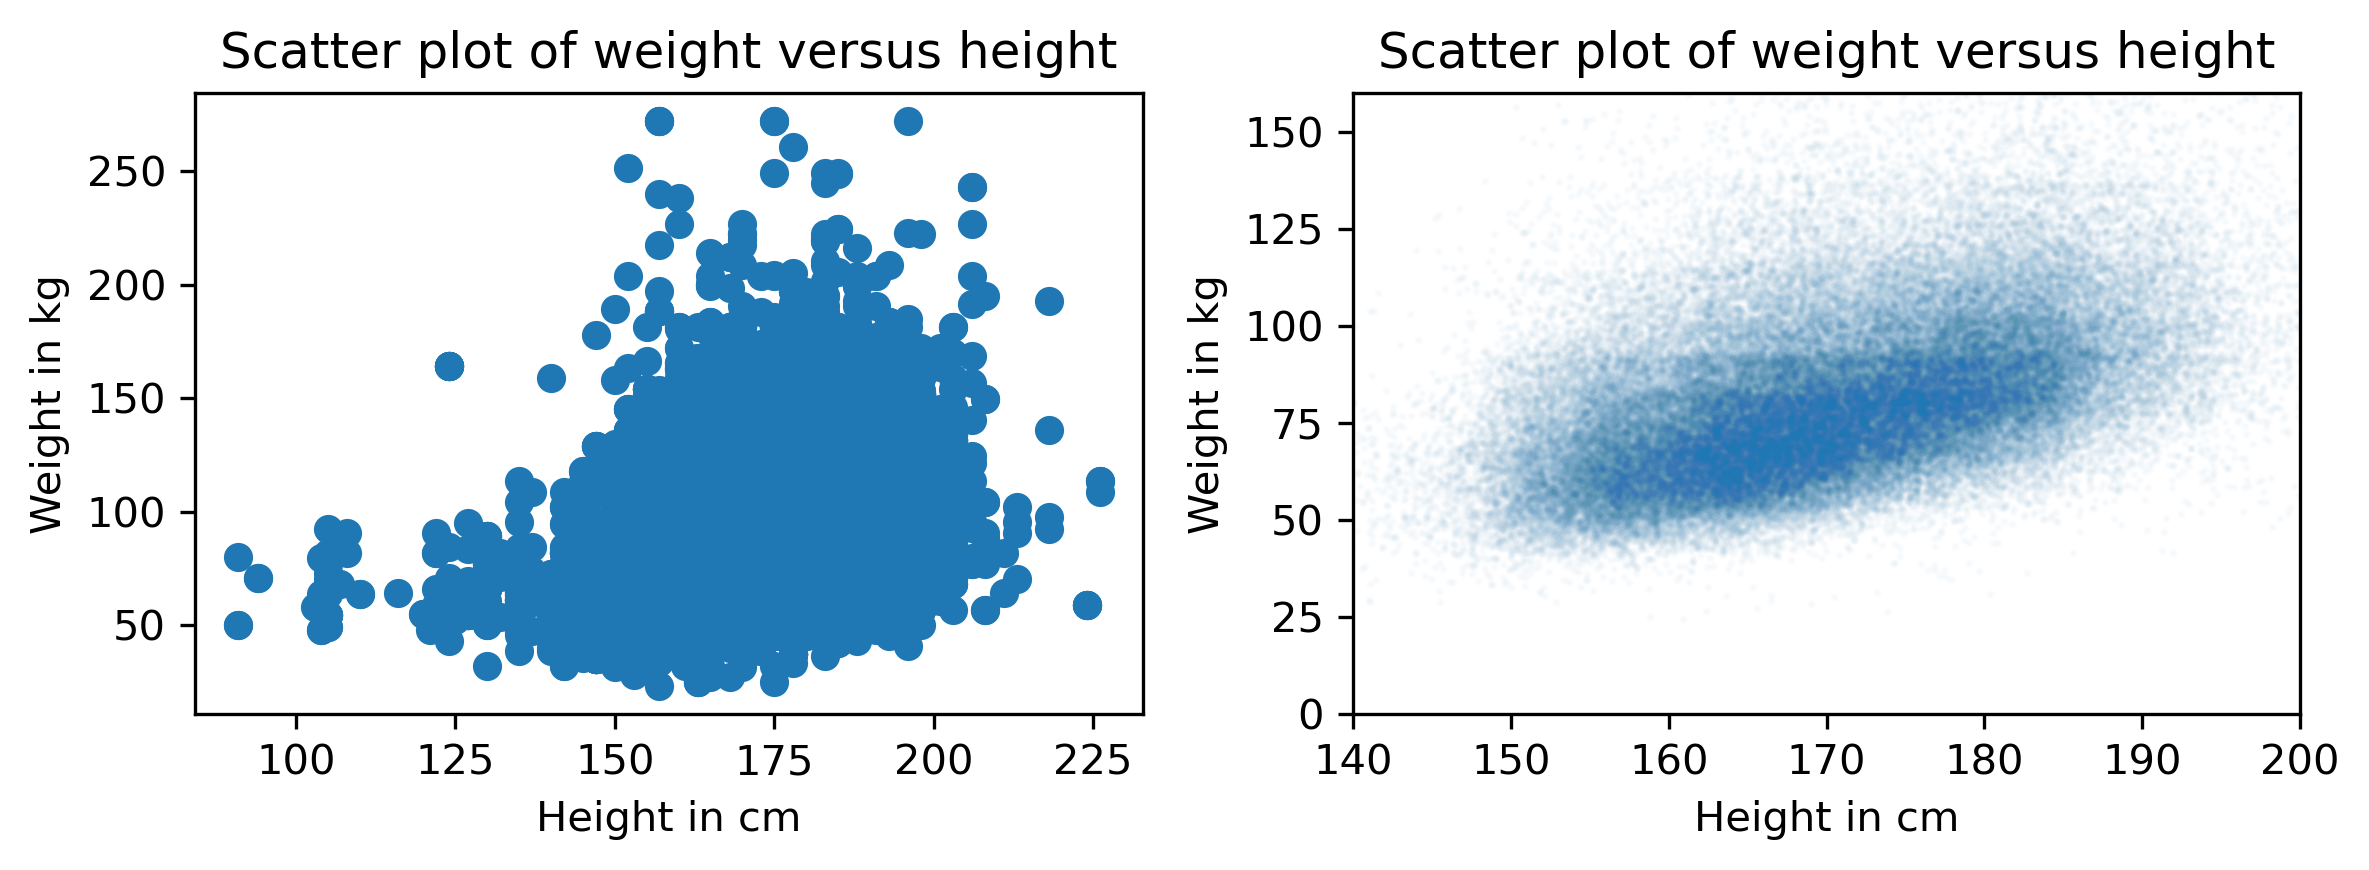
\includegraphics[width=4in]{chapters/09_relationships_files/09_relationships_28_0.png}
\end{center}

Now we have a reliable picture of the relationship between height and
weight. Below you can see the misleading plot we started with and the
more reliable one we ended with. They are clearly different, and they
suggest different relationships between these variables.

\begin{lstlisting}[language=Python,style=source]
\end{lstlisting}

\begin{center}
\includegraphics[width=4in]{chapters/09_relationships_files/09_relationships_30_0.png}
\end{center}

The point of this example is that it takes some effort to make an
effective scatter plot.

\textbf{Exercise:} Do people tend to gain weight as they get older? We
can answer this question by visualizing the relationship between weight
and age. But before we make a scatter plot, it is a good idea to
visualize distributions one variable at a time. So let's look at the
distribution of age.

The BRFSS dataset includes a column, \passthrough{\lstinline!AGE!},
which represents each respondent's age in years. To protect respondents'
privacy, ages are rounded off into 5-year bins. The values in
\passthrough{\lstinline!AGE!} are the midpoints of the bins.

\begin{itemize}
\item
  Extract the variable \passthrough{\lstinline!'AGE'!} from
  \passthrough{\lstinline!brfss!} and assign it to
  \passthrough{\lstinline!age!}.
\item
  Plot the PMF of \passthrough{\lstinline!age!} as a bar chart, using
  \passthrough{\lstinline!Pmf!} from
  \passthrough{\lstinline!empiricaldist!}.
\end{itemize}

\textbf{Exercise:} Now let's look at the distribution of weight. The
column that contains weight in kilograms is
\passthrough{\lstinline!WTKG3!}. Because this column contains many
unique values, displaying it as a PMF doesn't work very well. Instead,
use \passthrough{\lstinline!Cdf!} from
\passthrough{\lstinline!empiricaldist!} to plot the CDF of weight.

\textbf{Exercise:} Now make a scatter plot of
\passthrough{\lstinline!weight!} versus \passthrough{\lstinline!age!}.
Adjust \passthrough{\lstinline!alpha!} and
\passthrough{\lstinline!markersize!} to avoid overplotting. Use
\passthrough{\lstinline!ylim!} to limit the y-axis from 0 to 200
kilograms.

\textbf{Exercise:} In the previous exercise, the ages fall in columns
because they've been rounded into 5-year bins. If we jitter them, the
scatter plot will show the relationship more clearly.

\begin{itemize}

\item
  Add random noise to \passthrough{\lstinline!age!} with mean
  \passthrough{\lstinline!0!} and standard deviation
  \passthrough{\lstinline!2.5!}.
\item
  Make a scatter plot and adjust \passthrough{\lstinline!alpha!} and
  \passthrough{\lstinline!markersize!} again.
\end{itemize}

\section{Visualizing relationships}\label{visualizing-relationships}

In the previous section we used scatter plots to visualize the
relationship between weight and height. In this section, we'll explore
the relationship between weight and \emph{age}, and we'll see two new
ways to visualize relationships: box plots and violin plots.

Let's start with a scatter plot.

\begin{lstlisting}[language=Python,style=source]
age = brfss['AGE']
noise = np.random.normal(0, 1.0, size=len(brfss))
age_jitter = age + noise

plt.plot(age_jitter, weight_jitter, 'o', alpha=0.01, markersize=0.5)

plt.xlabel('Age in years')
plt.ylabel('Weight in kg')
plt.title('Weight versus age');
\end{lstlisting}

\begin{center}
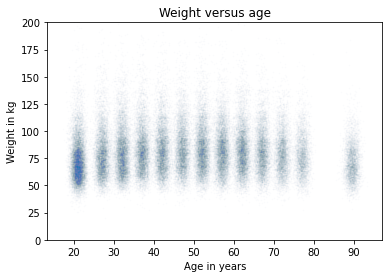
\includegraphics[width=4in]{chapters/09_relationships_files/09_relationships_39_0.png}
\end{center}

The ages are jittered, but the standard deviation of the noise is small
enough that there's still space between the columns. That makes it
possible to see the shape of the distribution in each age group, as well
as the differences between groups.

If we take this idea one step farther, we can use KDE to estimate the
density function in each column and plot it. This way of visualizing the
data is called a \textbf{violin plot}. Seaborn provides a function that
makes violin plots, but before we can use it, we have to get rid of any
rows with missing data. Here's how:

\begin{lstlisting}[language=Python,style=source]
data = brfss.dropna(subset=['AGE', 'WTKG3'])
data.shape
\end{lstlisting}

\begin{lstlisting}[style=output]
(393080, 10)
\end{lstlisting}

\passthrough{\lstinline!dropna!} creates a new
\passthrough{\lstinline!DataFrame!} that omits the rows in
\passthrough{\lstinline!brfss!} where \passthrough{\lstinline!AGE!} or
\passthrough{\lstinline!WTKG3!} are \passthrough{\lstinline!NaN!}. Now
we can call \passthrough{\lstinline!violinplot!} like this:

\begin{lstlisting}[language=Python,style=source]
import seaborn as sns

sns.violinplot(x='AGE', y='WTKG3', data=data, inner=None)

plt.xlabel('Age in years')
plt.ylabel('Weight in kg')
plt.title('Weight versus age');
\end{lstlisting}

\begin{center}
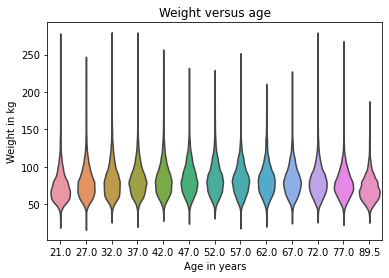
\includegraphics[width=4in]{chapters/09_relationships_files/09_relationships_43_0.png}
\end{center}

The \passthrough{\lstinline!x!} and \passthrough{\lstinline!y!}
arguments are the names of columns from \passthrough{\lstinline!data!},
which is the \passthrough{\lstinline!DataFrame!} we just created. The
argument \passthrough{\lstinline!inner=None!} simplifies the plot. In
the result each shape shows the distribution of weight in one age group.
The width of each shape is proportional to the estimated density, so
it's like two vertical KDEs plotted back to back.

Another, related way to look at data like this is called a \textbf{box
plot}, which shows summary statistics of the values in each group.
Seaborn provides a function that makes box plots -- we can call it like
this:

\begin{lstlisting}[language=Python,style=source]
sns.boxplot(x='AGE', y='WTKG3', data=data, whis=10)

plt.xlabel('Age in years')
plt.ylabel('Weight in kg')
plt.title('Weight versus age');
\end{lstlisting}

\begin{center}
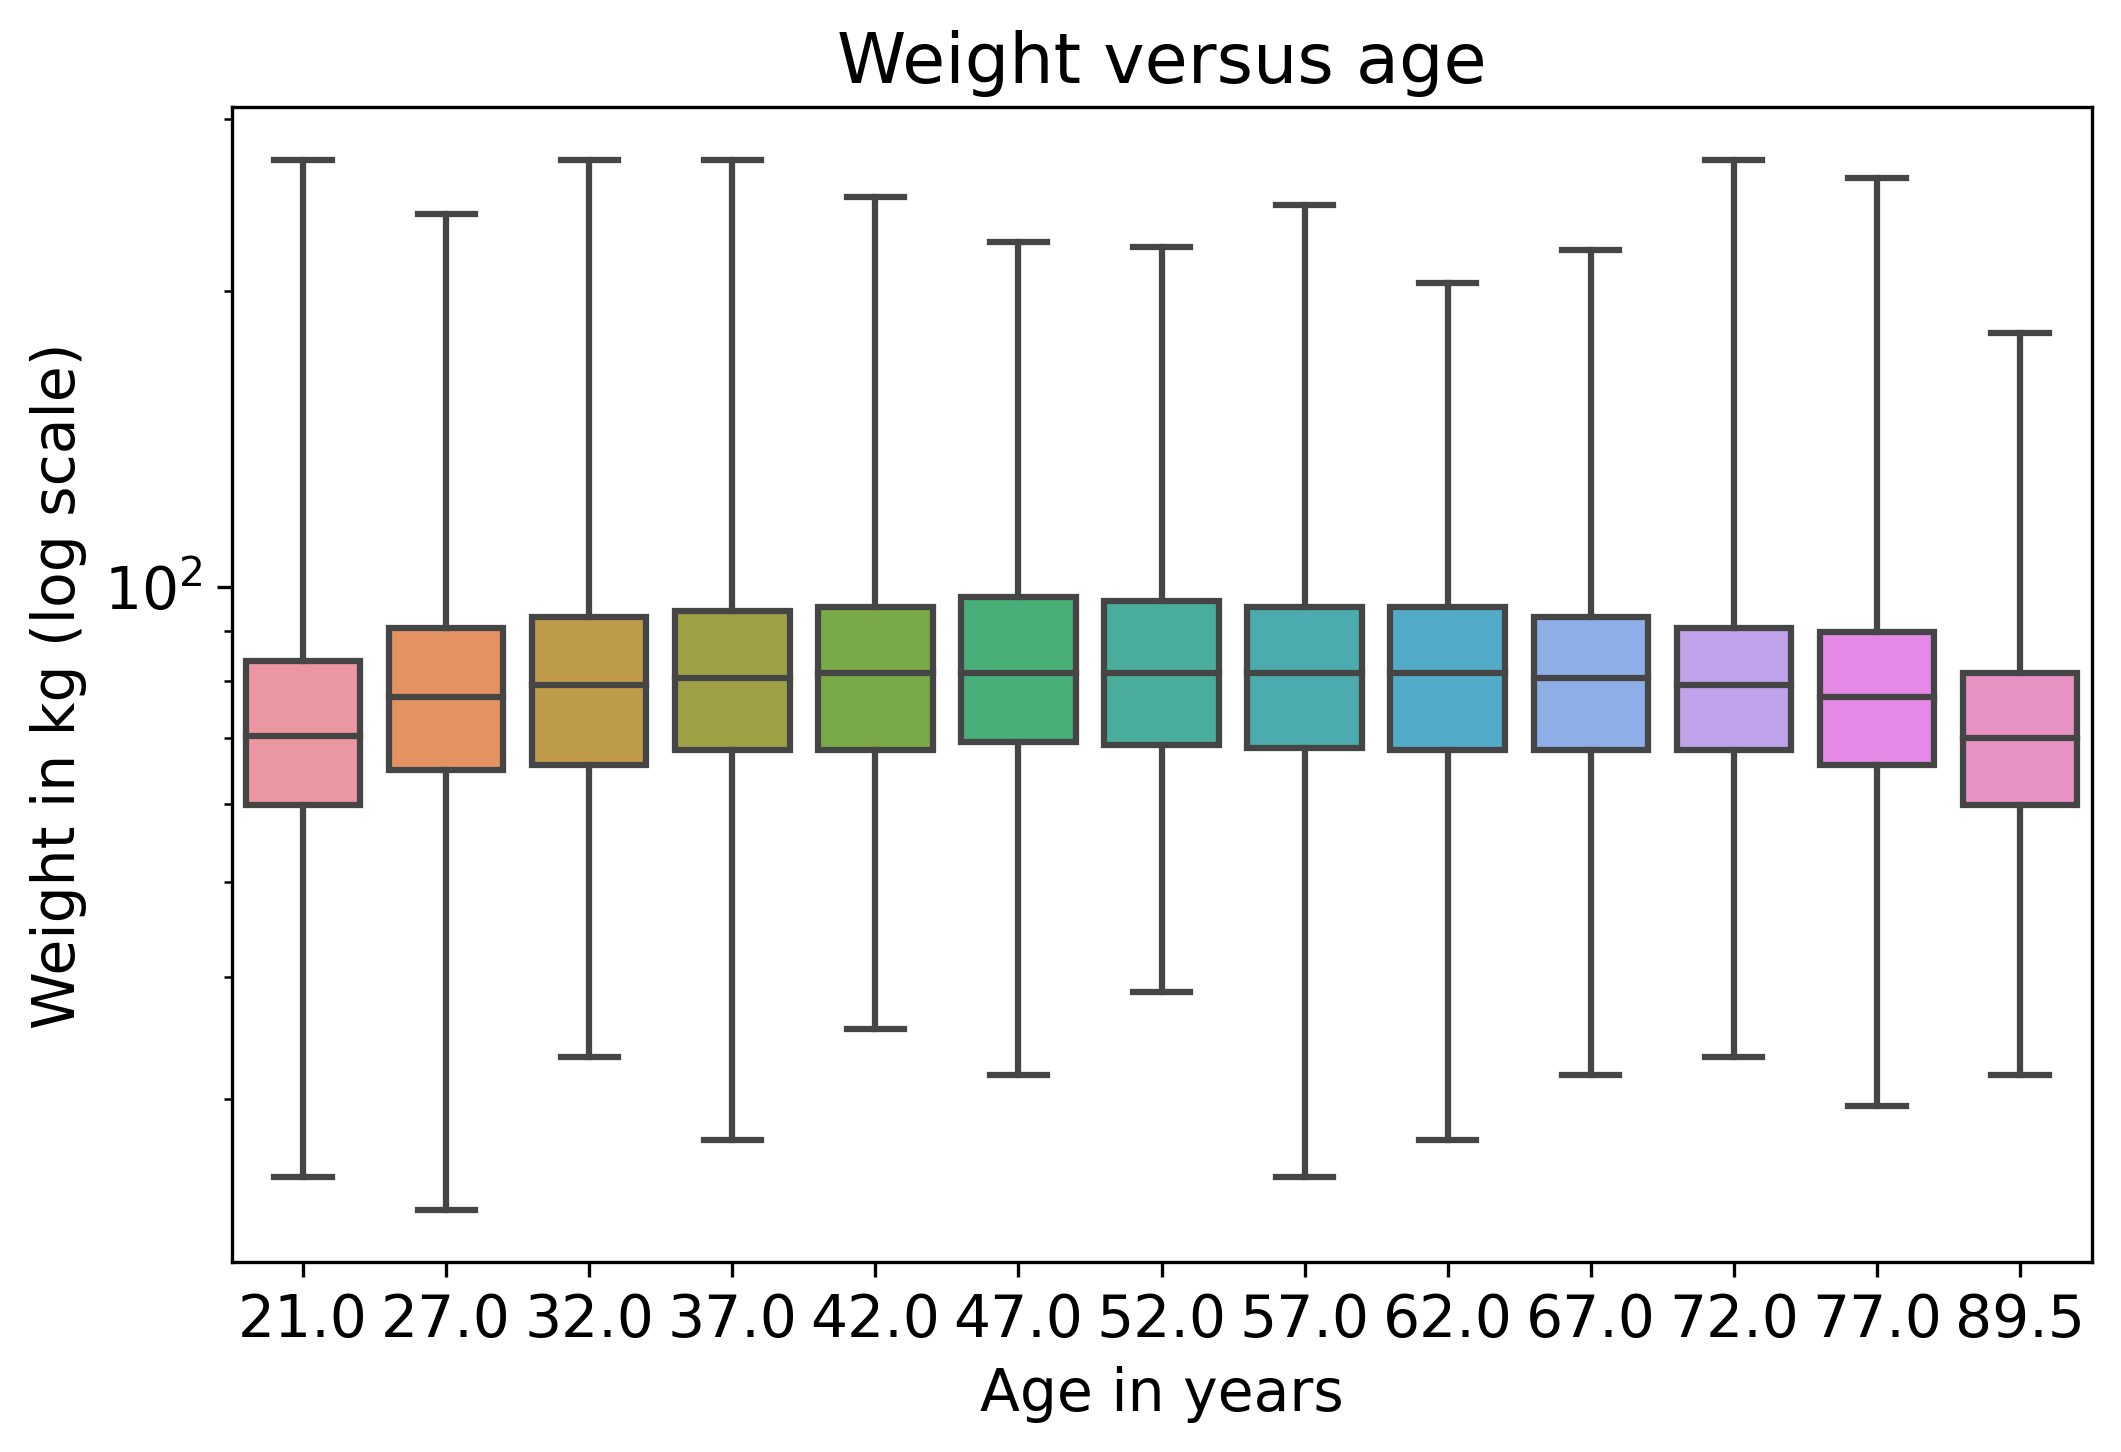
\includegraphics[width=4in]{chapters/09_relationships_files/09_relationships_46_0.png}
\end{center}

Each box represents the distribution of weight in an age group. The
height of each box represents the interquartile range, which is the
range from the 25th to the 75th percentile. The line in the middle of
each box is the median.

The keyword argument \passthrough{\lstinline!whis!} determines the
behavior of the whiskers that extend above and below the boxes. With
\passthrough{\lstinline!whis=10!}, they extend far enough to show the
minimum and maximum values.

In my opinion, this plot gives us the best view of the relationship
between weight and age.

\begin{itemize}
\item
  Looking at the medians, we can see that people in their 40s are the
  heaviest; younger and older people are lighter.
\item
  Looking at the sizes of the boxes, it seems like people in their 40s
  have the most variability in weight, too.
\item
  Looking at the whiskers, we can see that the distribution of weight is
  skewed -- that is, the heaviest people are farther from the median
  than the lightest people.
\end{itemize}

When a distribution is skewed toward higher values, it is sometimes
useful to plot it on a logarithmic scale. We can do that with the Pyplot
function \passthrough{\lstinline!yscale!}.

\begin{lstlisting}[language=Python,style=source]
sns.boxplot(x='AGE', y='WTKG3', data=data, whis=10)

plt.yscale('log')
plt.xlabel('Age in years')
plt.ylabel('Weight in kg (log scale)')
plt.title('Weight versus age');
\end{lstlisting}

\begin{center}
\includegraphics[width=4in]{chapters/09_relationships_files/09_relationships_49_0.png}
\end{center}

On a log scale, the distributions are symmetric, so the whiskers extend
about the same distance in both directions, the boxes are close to the
middle of the figure, and we can see the relationship between age and
weight clearly.

In the following exercises, you can generate violin and box plots for
other variables.

\textbf{Exercise:} Previously we looked at a scatter plot of height and
weight, and saw that taller people tend to be heavier. Now let's take a
closer look using a box plot. The \passthrough{\lstinline!brfss!}
DataFrame contains a column named \passthrough{\lstinline!\_HTMG10!}
that represents height in centimeters, binned into 10 cm groups.

\begin{itemize}
\item
  Make a box plot that shows the distribution of weight in each height
  group.
\item
  Plot the y-axis on a logarithmic scale.
\end{itemize}

Suggestion: If the labels on the x-axis collide, you can rotate them
with \passthrough{\lstinline!plt.xticks(rotation=45)!}.

\textbf{Exercise:} As a second example, let's look at the relationship
between income and height. In the BRFSS, income is represented as a
categorical variable -- that is, respondents are assigned to one of
seven income categories. The column name is
\passthrough{\lstinline!\_INCOMG1!}. Before we connect income with
anything else, let's look at the distribution by computing the PMF.
Extract \passthrough{\lstinline!\_INCOMG1!} from
\passthrough{\lstinline!brfss!} and assign it to
\passthrough{\lstinline!income!}. Then plot the PMF of
\passthrough{\lstinline!income!} as a bar chart.

\textbf{Exercise:} Generate a violin plot that shows the distribution of
height in each income group. Can you see a relationship between these
variables?

\section{Quantifying Correlation}\label{quantifying-correlation}

In the previous section, we visualized relationships between pairs of
variables. Now we'll quantify the strength of those relationships by
computing their correlation.

When people say ``correlation'' casually, they might mean any
relationship between two variables. In statistics, it usually means a
\textbf{correlation coefficient}, which is a number between -1 and 1
that quantifies the strength of a linear relationship between variables.
To demonstrate, we'll select three columns from the BRFSS dataset:

\begin{lstlisting}[language=Python,style=source]
columns = ['HTM4', 'WTKG3', 'AGE']
subset = brfss[columns]
\end{lstlisting}

The result is a \passthrough{\lstinline!DataFrame!} with just those
columns. With this subset of the data, we can use the
\passthrough{\lstinline!corr!} method, like this:

\begin{lstlisting}[language=Python,style=source]
subset.corr()
\end{lstlisting}

\begin{tabular}{lrrr}
\midrule
 & HTM4 & WTKG3 & AGE \\
\midrule
HTM4 & 1.000000 & 0.469398 & -0.122187 \\
WTKG3 & 0.469398 & 1.000000 & -0.067902 \\
AGE & -0.122187 & -0.067902 & 1.000000 \\
\midrule
\end{tabular}

The result is a \textbf{correlation matrix}. Reading across the first
row, the correlation of \passthrough{\lstinline!HTM4!} with itself is 1.
That's expected -- the correlation of anything with itself is 1.

The next entry is more interesting: the correlation of height and weight
is about 0.45. It's positive, which means taller people are heavier, and
it's moderate in strength, which means it has some predictive value --
if you know someone's height, you can make a somewhat better guess about
their weight.

The correlation between height and age is about -0.09. It's negative,
which means that older people tend to be shorter, but it's weak, which
means that knowing someone's age would not help much if you were trying
to guess their height.

Reading across the second row, we can see that the correlation of height
and weight is the same as the correlation of weight and height --
because correlation is commutative.

And we can see that the correlation of weight and age is only 0.001,
which is very small. It is tempting to conclude that there is no
relationship between age and weight, but we have already seen that there
is. So why is the correlation so low? Remember that the relationship
between weight and age looks like this.

\begin{lstlisting}[language=Python,style=source]
\end{lstlisting}

\begin{center}
\includegraphics[width=4in]{chapters/09_relationships_files/09_relationships_60_0.png}
\end{center}

As age increases, weight goes up and then down, so the relationship is
nonlinear. But correlation only measures linear relationships. When the
relationship is nonlinear, correlation generally underestimates how
strong it is.

To demonstrate this point more clearly, let's generate some fake data:
\passthrough{\lstinline!xs!} contains equally-spaced points between -1
and 1; \passthrough{\lstinline!ys!} is \passthrough{\lstinline!xs!}
squared plus some random noise.

\begin{lstlisting}[language=Python,style=source]
xs = np.linspace(-1, 1)
ys = xs**2 + np.random.normal(0, 0.05, len(xs))
\end{lstlisting}

Here's the scatter plot of these values.

\begin{lstlisting}[language=Python,style=source]
plt.plot(xs, ys, 'o', alpha=0.5)
plt.xlabel('x')
plt.ylabel('y')
plt.title('Scatter plot of a fake dataset');
\end{lstlisting}

\begin{center}
\includegraphics[width=4in]{chapters/09_relationships_files/09_relationships_64_0.png}
\end{center}

This is a strong relationship in the sense that you can make a much
better guess about \passthrough{\lstinline!y!} if you are given
\passthrough{\lstinline!x!}. But here's the correlation matrix:

\begin{lstlisting}[language=Python,style=source]
np.corrcoef(xs, ys)
\end{lstlisting}

\begin{lstlisting}[style=output]
array([[ 1.        , -0.01766183],
       [-0.01766183,  1.        ]])
\end{lstlisting}

Even though there is a strong non-linear relationship, the computed
correlation is close to zero. In general, if correlation is high -- that
is, close to 1 or -1 -- you can conclude that there is a strong linear
relationship. But if correlation is close to zero, that doesn't mean
there is no relationship; there might be a non-linear relationship. This
is one reason correlation can be misleading.

And there's another reason to be careful with correlation -- it doesn't
mean what people take it to mean. Specifically, correlation says nothing
about the slope of the line that fits the data. If we say that two
variables are correlated, that means we can use one to predict the
other. But that might not be what we care about.

For example, suppose we are concerned about the health effects of weight
gain, so we plot weight versus age from 20 to 50 years old. I'll
generate two fake datasets to demonstrate the point. In each dataset,
\passthrough{\lstinline!xs!} represents age and
\passthrough{\lstinline!ys!} represents weight.

\begin{lstlisting}[language=Python,style=source]
np.random.seed(18)
xs1 = np.linspace(20, 50)
ys1 = 75 + 0.02 * xs1 + np.random.normal(0, 0.15, len(xs1))
\end{lstlisting}

\begin{lstlisting}[language=Python,style=source]
np.random.seed(18)
xs2 = np.linspace(20, 50)
ys2 = 65 + 0.2 * xs2 + np.random.normal(0, 3, len(xs2))
\end{lstlisting}

Here's what the two scatter plots look like.

\begin{lstlisting}[language=Python,style=source]
plt.figure(figsize=(10, 3.5))

plt.subplot(1, 2, 1)
plt.plot(xs1, ys1, 'o', alpha=0.5)
plt.xlabel('Age in years')
plt.ylabel('Weight in kg')
plt.title('Fake dataset #1')
plt.tight_layout()

plt.subplot(1, 2, 2)
plt.plot(xs2, ys2, 'o', alpha=0.5)
plt.xlabel('Age in years')
plt.ylabel('Weight in kg')
plt.title('Fake dataset #2')
plt.tight_layout()
\end{lstlisting}

\begin{center}
\includegraphics[width=4in]{chapters/09_relationships_files/09_relationships_72_0.png}
\end{center}

I constructed these examples so they look similar, but they have
substantially different correlations.

\begin{lstlisting}[language=Python,style=source]
rho1 = np.corrcoef(xs1, ys1)[0, 1]
rho1
\end{lstlisting}

\begin{lstlisting}[style=output]
0.7579660563439401
\end{lstlisting}

\begin{lstlisting}[language=Python,style=source]
rho2 = np.corrcoef(xs2, ys2)[0, 1]
rho2
\end{lstlisting}

\begin{lstlisting}[style=output]
0.4782776976576317
\end{lstlisting}

In the first dataset, the correlation is strong, close to 0.75. In the
second dataset, the correlation is moderate, close to 0.5. So we might
think the first relationship is more important. But look more closely at
the y-axis in both figures.

In the first example, the average weight gain over 30 years is less than
1 kilogram; in the second it is more than 5 kilograms! If we are
concerned about the health effects of weight gain, the second
relationship is probably more important, even though the correlation is
lower. In this scenario, the statistic we really care about is the slope
of the line that fits the data, not the coefficient of correlation. In
the next section, we'll use linear regression to compute that slope, but
first let's practice with correlation.

\textbf{Exercise:} The purpose of the BRFSS is to explore health risk
factors, so it includes questions about diet. The column
\passthrough{\lstinline!\_VEGESU1!} represents the number of servings of
vegetables respondents reported eating per day. Before we compute
correlations, let's look at the distribution of this variable. Extract
\passthrough{\lstinline!\_VEGESU1!} from \passthrough{\lstinline!brfss!}
and assign it to \passthrough{\lstinline!vegesu!} -- then plot the CDF
of the values.

The original dataset includes a small number of values greater than 10,
some of them unreasonably large. For this extract, I have cut off the
values at 10.

\textbf{Exercise:} Now let's visualize the relationship between age and
vegetables. Make a box plot that summarizes the distribution of
vegetable servings in each age group. How would you describe the
relationship, if any?

\textbf{Exercise:} Finally, let's look at correlations between age,
income, and vegetable servings.

\begin{itemize}

\item
  From \passthrough{\lstinline!brfss!}, select the columns
  \passthrough{\lstinline!'AGE'!}, \passthrough{\lstinline!\_INCOMG1!},
  and \passthrough{\lstinline!\_VEGESU1!}.
\item
  Compute the correlation matrix for these variables.
\end{itemize}

Is the correlation between age and vegetable servings what you expected
based on the box plot?

\section{Simple Linear Regression}\label{simple-linear-regression}

In the previous section we saw that correlation does not always measure
what we really want to know. In this section, we look at an alternative:
simple linear regression. Here ``simple'' means there are only two
variables, as opposed to ``multiple'' regression, which can work with
any number of variables.

In the previous section, I generated fake datasets showing two
hypothetical relationships between weight and age. We computed
correlations for both datasets, now let's compute lines of best fit. We
can use \passthrough{\lstinline!linregress!} from the SciPy
\passthrough{\lstinline!stats!} library, which takes two sequences as
arguments. Here are the results for Fake Dataset \#1.

\begin{lstlisting}[language=Python,style=source]
from scipy.stats import linregress

res1 = linregress(xs1, ys1)
res1._asdict()
\end{lstlisting}

\begin{lstlisting}[style=output]
{'slope': 0.018821034903244386,
 'intercept': 75.08049023710964,
 'rvalue': 0.7579660563439402,
 'pvalue': 1.8470158725246148e-10,
 'stderr': 0.002337849260560818,
 'intercept_stderr': 0.08439154079040358}
\end{lstlisting}

The result is a \passthrough{\lstinline!LinregressResult!} object that
contains five values: \passthrough{\lstinline!slope!} is the slope of
the line of best fit for the data, \passthrough{\lstinline!intercept!}
is the intercept, and \passthrough{\lstinline!rvalue!} is correlation.
We'll ignore the other values for now.

For Fake Dataset \#1, the estimated slope is about 0.019 kilograms per
year or about 0.56 kilograms over the 30-year range.

\begin{lstlisting}[language=Python,style=source]
res1.slope * 30
\end{lstlisting}

\begin{lstlisting}[style=output]
0.5646310470973316
\end{lstlisting}

Here are the results for Fake Dataset \#2.

\begin{lstlisting}[language=Python,style=source]
res2 = linregress(xs2, ys2)
res2._asdict()
\end{lstlisting}

\begin{lstlisting}[style=output]
{'slope': 0.17642069806488855,
 'intercept': 66.60980474219305,
 'rvalue': 0.47827769765763173,
 'pvalue': 0.0004430600283776241,
 'stderr': 0.04675698521121631,
 'intercept_stderr': 1.6878308158080697}
\end{lstlisting}

The estimated slope is almost 10 times higher, about 0.18 kilograms per
year or about 5.3 kilograms per 30 years.

\begin{lstlisting}[language=Python,style=source]
res2.slope * 30
\end{lstlisting}

\begin{lstlisting}[style=output]
5.292620941946657
\end{lstlisting}

We can use the results from \passthrough{\lstinline!linregress!} to plot
the line of best fit and see how it relates to the data. First we get
the minimum and maximum of the observed \passthrough{\lstinline!xs!}.
Then we multiply by the slope and add the intercept.

\begin{lstlisting}[language=Python,style=source]
low, high = xs1.min(), xs1.max()
fx = np.array([low, high])
fy = res1.intercept + res1.slope * fx
\end{lstlisting}

Here's what the result looks like for the first example.

\begin{lstlisting}[language=Python,style=source]
plt.plot(xs1, ys1, 'o', alpha=0.5)
plt.plot(fx, fy, '-')

plt.xlabel('Age in years')
plt.ylabel('Weight in kg')
plt.title('Fake Dataset #1');
\end{lstlisting}

\begin{center}
\includegraphics[width=4in]{chapters/09_relationships_files/09_relationships_91_0.png}
\end{center}

We can do the same thing for the second example.

\begin{lstlisting}[language=Python,style=source]
low, high = xs2.min(), xs2.max()
fx = np.array([low, high])
fy = res2.intercept + res2.slope * fx
\end{lstlisting}

And here's what the result looks like.

\begin{lstlisting}[language=Python,style=source]
plt.plot(xs2, ys2, 'o', alpha=0.5)
plt.plot(fx, fy, '-')

plt.xlabel('Age in years')
plt.ylabel('Weight in kg')
plt.title('Fake Dataset #2');
\end{lstlisting}

\begin{center}
\includegraphics[width=4in]{chapters/09_relationships_files/09_relationships_95_0.png}
\end{center}

At first glance it might seem like the slope is steeper in the first
figure, but don't be fooled. If you look closely at the vertical scales,
the slope in the second figure is almost 10 times higher.

\section{Regression of Height and
Weight}\label{regression-of-height-and-weight}

Now let's look at an example of regression with real data. Here's the
scatter plot of height and weight one more time.

\begin{lstlisting}[language=Python,style=source]
plt.plot(height_jitter, weight_jitter, 'o', 
         alpha=0.01, markersize=0.5)

plt.xlim([140, 200])
plt.ylim([0, 160])
plt.xlabel('Height in cm')
plt.ylabel('Weight in kg')
plt.title('Scatter plot of weight versus height');
\end{lstlisting}

\begin{center}
\includegraphics[width=4in]{chapters/09_relationships_files/09_relationships_98_0.png}
\end{center}

To compute the regression line, we'll use
\passthrough{\lstinline!linregress!} again. But it can't handle
\passthrough{\lstinline!NaN!} values, so we have to use
\passthrough{\lstinline!dropna!} to remove rows that are missing the
data we need.

\begin{lstlisting}[language=Python,style=source]
data = brfss.dropna(subset=['WTKG3', 'HTM4'])
\end{lstlisting}

Now we can compute the linear regression.

\begin{lstlisting}[language=Python,style=source]
res_hw = linregress(data['HTM4'], data['WTKG3'])
res_hw._asdict()
\end{lstlisting}

\begin{lstlisting}[style=output]
{'slope': 0.9366891536604244,
 'intercept': -76.44247680097321,
 'rvalue': 0.4693981914367916,
 'pvalue': 0.0,
 'stderr': 0.002806793650907722,
 'intercept_stderr': 0.47939863668166327}
\end{lstlisting}

The slope is about 0.9 kilograms per centimeter, which means that we
expect a person one centimeter taller to be almost a kilogram heavier.
That's quite a lot. As before, we can compute the line of best fit:

\begin{lstlisting}[language=Python,style=source]
low, high = data['HTM4'].min(), data['HTM4'].max()
fx = np.array([low, high])
fy = res_hw.intercept + res_hw.slope * fx
\end{lstlisting}

And here's what that looks like.

\begin{lstlisting}[language=Python,style=source]
plt.plot(height_jitter, weight_jitter, 'o', alpha=0.01, markersize=0.5)
plt.plot(fx, fy, '-')

plt.xlim([140, 200])
plt.ylim([0, 160])
plt.xlabel('Height in cm')
plt.ylabel('Weight in kg')
plt.title('Scatter plot of weight versus height');
\end{lstlisting}

\begin{center}
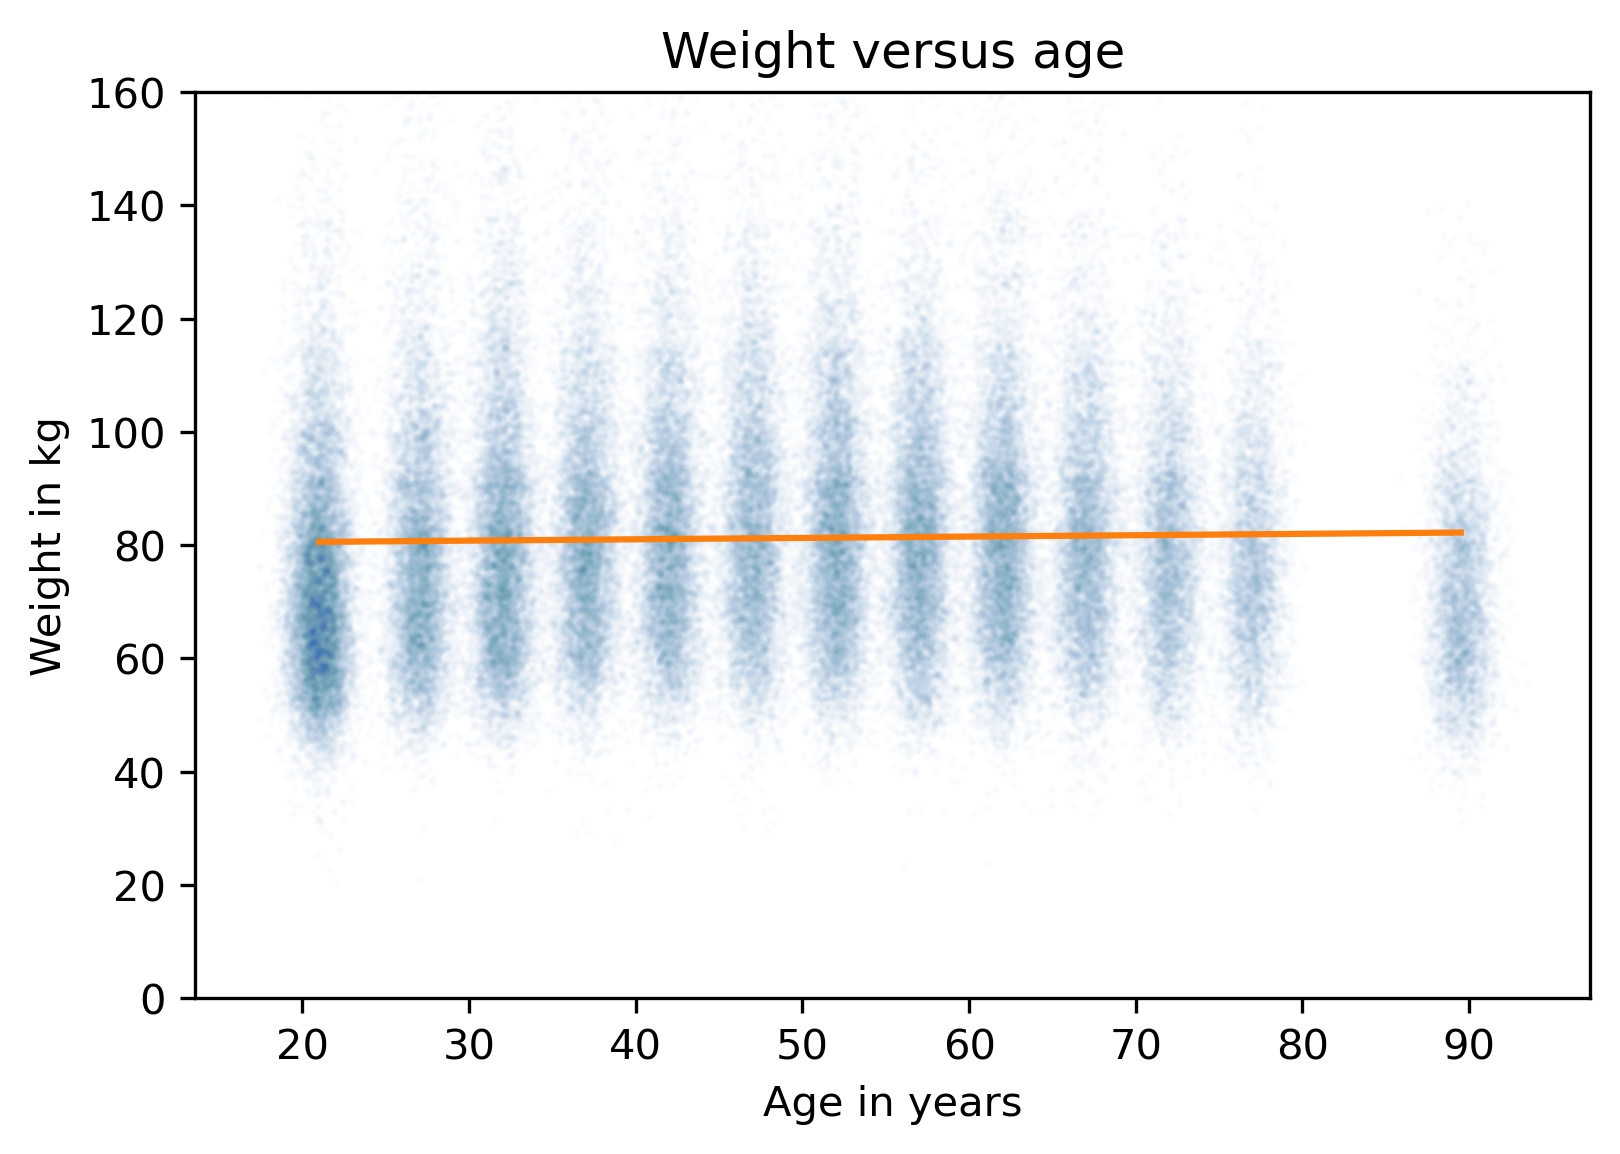
\includegraphics[width=4in]{chapters/09_relationships_files/09_relationships_106_0.png}
\end{center}

The slope of this line seems consistent with the scatter plot. As
another example, here's the scatter plot of weight versus age, which we
saw earlier.

\begin{lstlisting}[language=Python,style=source]
plt.plot(age_jitter, weight_jitter, 'o', 
         alpha=0.01, markersize=0.5)

plt.ylim([0, 160])
plt.xlabel('Age in years')
plt.ylabel('Weight in kg')
plt.title('Weight versus age');
\end{lstlisting}

\begin{center}
\includegraphics[width=4in]{chapters/09_relationships_files/09_relationships_108_0.png}
\end{center}

As we have seen before, the relationship is nonlinear. Let's see what we
get if we compute a linear regression.

\begin{lstlisting}[language=Python,style=source]
subset = brfss.dropna(subset=['WTKG3', 'AGE']) 
res_aw = linregress(subset['AGE'], subset['WTKG3'])
res_aw._asdict()
\end{lstlisting}

\begin{lstlisting}[style=output]
{'slope': -0.08138685042569352,
 'intercept': 87.66340016901641,
 'rvalue': -0.06790235862083926,
 'pvalue': 0.0,
 'stderr': 0.0019073328587490353,
 'intercept_stderr': 0.11019675319089409}
\end{lstlisting}

The estimated slope is close to zero. Here's what the line of best fit
looks like.

\begin{lstlisting}[language=Python,style=source]
plt.plot(age_jitter, weight_jitter, 'o', 
         alpha=0.01, markersize=0.5)

low, high = data['AGE'].min(), data['AGE'].max()
fx = np.array([low, high])
fy = res_aw.intercept + res_aw.slope * fx
plt.plot(fx, fy, '-')

plt.ylim([0, 160])
plt.xlabel('Age in years')
plt.ylabel('Weight in kg')
plt.title('Weight versus age');
\end{lstlisting}

\begin{center}
\includegraphics[width=4in]{chapters/09_relationships_files/09_relationships_112_0.png}
\end{center}

A straight line does not capture the relationship between these
variables well. That's because linear regression has the same problem as
correlation -- it only measures the strength of a linear relationship.

In the next chapter, we'll see how to use multiple regression to
quantify non-linear relationships. But first, let's practice using
simple regression.

\textbf{Exercise:} Who do you think eats more vegetables, people with
low income, or people with high income? Let's find out. As we've seen
previously, the column \passthrough{\lstinline!\_INCOMG1!} represents
income level and \passthrough{\lstinline!\_VEGESU1!} represents the
number of vegetable servings respondents reported eating per day. Make a
scatter plot with vegetable servings versus income, that is, with
vegetable servings on the y-axis and income group on the x-axis. You
might want to use \passthrough{\lstinline!ylim!} to zoom in on the
bottom half of the y-axis.

\textbf{Exercise:} Now estimate the slope of the relationship between
vegetable consumption and income.

\begin{itemize}
\item
  Use \passthrough{\lstinline!dropna!} to select rows where
  \passthrough{\lstinline!\_INCOMG1!} and
  \passthrough{\lstinline!\_VEGESU1!} are not
  \passthrough{\lstinline!NaN!}.
\item
  Extract \passthrough{\lstinline!\_INCOMG1!} and
  \passthrough{\lstinline!\_VEGESU1!} and compute the simple linear
  regression of these variables.
\item
  Finally, plot the regression line on top of the scatter plot.
\end{itemize}

What is the slope of the regression line? What does this slope means in
the context of the question we are exploring?

\section{Summary}\label{summary}

This chapter presents three ways to visualize the relationship between
two variables: a scatter plot, violin plot, and box plot. A scatter plot
is often a good choice when you are exploring a new data set, but it can
take some attention to avoid overplotting. Violin plots and box plots
are particularly useful when one of the variables has only a few unique
values or the values have been rounded into bins.

We considered two ways to quantify the strength of a relationship: the
coefficient of correlation and the slope of a regression line. These
statistics capture different aspect of what we might mean by
``strength''. The coefficient of correlation indicates how well we can
predict one variable, given the other. The slope of the regression line
indicates how much difference we expect in one variable as we vary the
other. One or the other might be more relevant, depending on the
context.

